\section{Kodkod Architecture}
\label{sec:kodkod}

Kodkod was designed and implemented by Emina Torlak as part of her PhD thesis
 under Daniel Jackson at MIT~\cite{t-dissertation-2009}.
Her thesis and \href{http://alloy.mit.edu/kodkod/release/current/doc/}{Java implemention} were the primary guides for my work.

Kodkod is a solver for relational logic designed to effectively utilize partial solutions.
Relational logic is first-order logic extended with a handful of so-called relational operators
 to express properties like the transpose and closure of bounded variables.
%\begin{itemize}
%\item $\sim e$ is the transpose of the expression $e$
%\item $\hat{}e$ is the transitive closure of $e$
%\item $* e$ is the reflexive closure of $e$
%\end{itemize}
There are three key assumptions supporting Kodkod's design:
\begin{itemize}
\item Relational logic is well-suited for describing engineering problems.
   For instance, transitive closure can describe reachability in a graph.
\item Engineers often have access to partial solutions, informations from
   which should be used the guide the search for a full solution.
\item Modern SAT solvers are extremely fast, to the point that compiling
   a high-level logic to SAT queries is competitive with compiling to SMT.
\end{itemize}

We assume these are still valid, but it would be interesting to compare
 today's SAT and SMT solvers and perhaps reproduce the earlier results that
 SAT was arguably the better choice.

The high-level architecture of Kodkod is show in \figref{fig:arch}.
Input from the user, represented on the left of the figure, comes in three
 required forms.
First is a listing of the \emph{atoms} over which the problem and its solutions
 will be expressed.
These are a finite set of otherwise arbitrary symbols.
Second are \emph{relational bounds} expressed in terms of the atoms.
Each relational bound is an identifier {\tt ID} and two sets of tuples of atoms\textemdash
 in other words, two relations on atoms.
The first relation is a lower bound and expresses the relations that must
 be included in {\tt ID}.
The second relation is an upper bound and expresses relations that might be
 in {\tt ID}.
The lower and upper bounds must contain tuples of the same arity.
Also the lower bound must be contained in the upper bound.
For example, given the atoms {\tt\{true, false\}}
 the type {\tt Boolean} can be encoded by giving {\tt\{(true, false)\}} as
 both the upper and lower bound.
Third are formulas over the atoms and variables written in relational logic.
These formulas may be constraints in the problem or partial solutions.

The second phase of Kodkod, shown in the middle of the figure, is a translation
 from relational logic to an intermediate representation of boolean matrices.
First existential variables are Skolemized up to a user-determined depth.
Then relations $R$ over the $N$ atoms of the problem are encoded as $N \times N$
 matrices where the entry at row $i$ and column $j$ is 1 iff the pair of atoms
 $(i, j)$ is in the relation $R$.
Similarly, relational bounds of arity $k$ are encoded as $k$-dimensional matrices
 using boolean variables as unknowns.

Two important optimizations occur at this stage.
First, the matrices are represented sparsely because most relations in a problem
 deal with only a few atoms.
Second, matrices are compacted using a technique by Torlak~\cite{t-dissertation-2009}
 for detecting symmetries and sharing data.

After a problem is converted to a compact boolean form, it is compiled to a boolean
 circuit and then translated to CNF for a solver.
The data is then fed to an off-the-shelf SAT solver.
If the solver proves the formula, all is well.
If not, we use a final key ingredient of Kodkod: minimal core extraction.
From the solver's proof of unsatisfiability Kodkod infers a minimal counterexample
 to the specification and presents it to the user.
In practice, this makes using the solver must less frustrating.

\begin{figure}
  \label{fig:arch}
  \begin{center}
  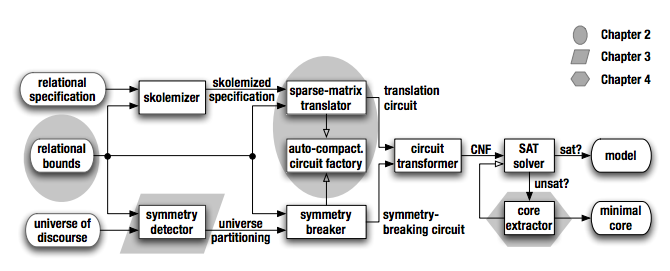
\includegraphics[width=12cm]{arch.png}
  \end{center}
  \caption{Kodkod architecture}
\end{figure}


